% AEJ-Article.tex for AEA last revised 22 June 2011
\documentclass[PP]{AEA}

%%%%%% NOTE FROM OVERLEAF: The mathtime package is no longer publicly available nor distributed. We recommend using a different font package e.g. mathptmx if you'd like to use a Times font.
\usepackage{mathptmx}

% The mathtime package uses a Times font instead of Computer Modern.
% Uncomment the line below if you wish to use the mathtime package:
%\usepackage[cmbold]{mathtime}https://www.overleaf.com/project/5de54d6638f785000167866a
% Note that miktex, by default, configures the mathtime package to use commercial fonts
% which you may not have. If you would like to use mathtime but you are seeing error
% messages about missing fonts (mtex.pfb, mtsy.pfb, or rmtmi.pfb) then please see
% the technical support document at http://www.aeaweb.org/templates/technical_support.pdf
% for instructions on fixing this problem.

% Note: you may use either harvard or natbib (but not both) to provide a wider
% variety of citation commands than latex supports natively. See below.

% Uncomment the next line to use the natbib package with bibtex 
\usepackage{url}
\usepackage{natbib}
\usepackage{hyperref}
\usepackage{acronym}
\usepackage[names]{xcolor}
\usepackage{graphicx}
\usepackage{csvsimple}
% Uncomment the next line to use the harvard package with bibtex
%\usepackage[abbr]{harvard}
\usepackage{etoolbox}
\usepackage{geometry}
\usepackage{caption} % to re-use counters

\newtoggle{fancy}
\togglefalse{fancy}

\newtoggle{draft}
\toggletrue{draft}
%\togglefalse{draft}

\newtoggle{final}
%\togglefalse{final}
\toggletrue{final}
%\iftoggle{final}{\togglefalse{draft}}{}


\iftoggle{draft}{
\usepackage{draftwatermark}
\SetWatermarkText{DRAFT}
\SetWatermarkScale{0.5}
\SetWatermarkLightness{0.85}%
}{\usepackage[final]{draftwatermark}}

\usepackage{xspace}
% to adjust floats
\usepackage{placeins}
% to read the table
\usepackage{booktabs}
\usepackage{ifthen}
\usepackage{csvsimple}
\usepackage{longtable}

\usepackage{textcomp}

\iftoggle{fancy}{
\input{fancy-config.tex}
}{}

\iftoggle{final}{
\usepackage[disable]{todonotes}
\newcommand{\misscitep}[2]{\citep{#2}}
\newcommand{\misscitet}[2]{\citet{#2}}
}{
\usepackage{todonotes}
\geometry{verbose,letterpaper,
	tmargin=1in,bmargin=1in,lmargin=1in,rmargin=2in}
\setlength{\marginparwidth}{1.9in}
\newcommand{\misscitep}[2]{\todo[color=green]{Missing citation: #1}{(\textcolor{red}{#2})}}
\newcommand{\misscitet}[2]{\todo[color=green]{Missing citation: #1}{\textcolor{red}{#2}}}
}



% This command determines the leading (vertical space between lines) in draft mode
% with 1.5 corresponding to "double" spacing.
\draftSpacing{1.5}

%% make somewhat tigher enumeration environments
\usepackage{enumitem}
\setlist[enumerate]{itemsep=0pt,parsep=0pt,topsep=1pt}
\setlist[itemize]{itemsep=0pt,parsep=0pt}

%% Acronyms
\acrodef{AEA}{American Economic Association}
\acrodef{DOI}{Digital Object Identifier}
\acrodef{FAIR}{Findable, Accessible, Interoperable, Re-usable}
\acrodef{PSID}{Panel Study of Income Dynamics}
\acrodef{HRS}{Health and Retirement Study}
\acrodef{RCT}{randomized control trial}
\acrodef{ICPSR}{Inter-university Consortium for Political and Social Research}
\acrodef{DCAP}{data and code availability policy}
\acrodef{PAP}{pre-analysis plans}
\acrodef{NACJD}{National Archive of Criminal Justice Data}
\acrodef{IAB}{Research Data Center (FDZ) at the Institute for Employment Research}
\acrodef{FSRDC}{Federal Statistical Research Data Centers}
\acrodef{FAQ}{frequently asked questions}
\acrodef{ReStud}{Review of Economic Studies}
\acrodef{EJ}{Economic Journal}
\acrodef{JASA}{Journal of the American Statistical Association}
\acrodef{CJE}{Canadian Journal of Economics}
\acrodef{AJPS}{American Journal of Political Science}
\acrodef{PII}{personally identifiable information}
\newcommand{\aeadcr}{AEA Data and Code Repository}

% reset colors
\definecolor{darkblue}{rgb}{0 0 255}
\hypersetup{colorlinks,breaklinks,citecolor=darkblue,linkcolor=darkblue,urlcolor=darkblue}

% Different ways to cite URLS
%\newcommand{\urlcite}[2]{\href{#1}{#2}
\newcommand{\urlcite}[2]{#2\footnote{\url{#1}}}
\newcommand{\furlcite}[2]{#2 (\url{#1})}

\begin{document}

\title{Report for 2020 by the AEA Data Editor }
\shortTitle{Report by Data Editor}
\author{Lars Vilhuber\thanks{%
Cornell University, lars.vilhuber@cornell.edu. }
}
\date{\today}
\pubMonth{May}
\pubYear{2020}
\pubVolume{--}
\pubIssue{--}
\JEL{}
\Keywords{reproducibility; replicability; science of science}




\maketitle

The \ac{AEA} Data Editor's  mission is to ``design  and  oversee  the  AEA  journals’  strategy for archiving and curating research data and promoting  reproducible  research'' \citep{10.1257/pandp.108.745}. The 2018 Report by the Data Editor \citep{10.1257/pandp.109.718} articulates how to implement that mission. Since July 2019, we have conducted comprehensive pre-publication reproducibility checks for all regular AEA journals, developed guidance for authors, and worked with peers at societies and groups in economics and elsewhere. 

Based on the experience from the first full year of reproducibility verification, we implemented several improvements in mid-2020. We provided improved guidance to authors depositing materials, clarified the \ac{DCAP}, expanded and clarified additional policies on third-party reproducibility checks, on post-publication updates to replication packages, and on required replication materials for field and lab experiments  (Section~\ref{sec:policies}). We have reached out to numerous data creators and providers --- both authors who have created unique data resources, and commercial data providers that often provide the data for economic research --- and have discussed with these data providers access to data for reproducibility checks, mechanisms to request publication approval, and generally informed them of the need for reproducibility, provenance tracing, and transparency in economic research (Section~\ref{sec:producers}). 
We continue to coordinate with other journals, societies, and registries on these topics (Section~\ref{sec:coordination}).

\begin{center}
	from here on, no changes yet
\end{center}

\section{Task 1: Reviewing the AEA Data and Code Availability Policy}
\label{sec:dcap}

After having introduced stronger principles of provenance and transparency into the  \ac{AEA}'s data and code availability policy in 2019 \citep{10.1257/pandp.110.dcap}, we monitored compliance and understanding as evidenced by the replication package submissions we received. It became quickly clear that stronger guidance, and greater clarity were needed to assist authors in complying with the \ac{DCAP}. Authors struggled with the concepts of data citations, how best to document their code and data, and with the process of deposing data and code. The results is a clarified policy, which we released in September 2020, and is reprinted in these proceedings \citep{10.1257/pandp.111.dcap}. We simplified the main policy,  separated out the policy as applied to papers conducting (field and lab) experiments, and expanded the policy to encompass more clearly any primary data collection. We also introduced  supplementary policies that lay out how and when we expect reproducibility checks by third-parties to be conducted, and, as a logical consequence of more transparent data and code deposits, how to revise data and code deposits when post-publication changes become necessary. These policies are reprinted in \citet{10.1257/pandp.111.dcap} and accessible online at \url{https://www.aeaweb.org/journals/data}.

We also clarified the data and code availability policy as it applies to these proceedings. All empirical and computational articles in the proceedings need to make code and data available in the same AEA Data and Code Repository as articles in the journals. However, other than verifying compliance with the policy (materials were deposited) and conducting basic checks (material can be read, metadata is in order), we do not conduct the same pre-publication reproducibility checks as we do for regular articles (see Section XXX for statistics on compliance).

But policies only outline what should occur. In order to assist authors in complying with the policy, thus improving turnaround times as well, we developed more detailed step-by-step guidance at \url{https://aeadataeditor.github.io/aea-de-guidance/step-by-step.html}. We also revised the information that authors need to provide when their manuscript is conditionally accepted (or, in some cases, during the review process). We have eliminated the duplicative requirement to provide  README files during the manuscript submission process --- they remain a required element in the data and code deposit process --- replacing it with a simpler form that requires authors to attest to compliance of their manuscript with the data citation requirement, provide details on where the data and code were deposited, and has them alert the Data Editor to any constraints on data access (we return to these access constraints in Section XXXX). A simplified version of the form (reduced to a few checkboxes) is incorporated into the initial manuscript submission workflow. The primary goal of these forms and checkboxes is to alert authors to the need to comply with the policy early on, and hopefully leading to better compliance by the time that manuscripts are conditionally accepted. 


\subsection{Improving Findability of Replication Materials at the AEA}
\label{sec:findability}

Since the AEA began using a data and code repository hosted by \ac{ICPSR}, all deposits have JEL codes, and authors can add funder information and key metadata describing the data that is available within the deposit. Many authors avail themselves of this option. These attributes aid in making each deposit  findable through scholarly search engines such as \urlcite{https://clarivate.com/webofsciencegroup/solutions/web-of-science/}{Web of Science} and \urlcite{https://scholar.google.com/}{Google Scholar}. 

Deposits made prior to July 2019 and since migrated to the AEA Data and Code Repository do not have the rich metadata, since it must be entered interactively by authors. To improve the metadata of older deposits, we ran a campaign in summer and fall of 2020, thanks to the support provided by a research team at the University of Michigan and ICPSR. This campaign targeted several hundred papers, providing authors with a tool to augment the metadata associated with their deposits. A report on the success of the campaign is forthcoming, and the metadata provided by the authors is being incorporated as this report was being compiled. A second campaign will complete the work in Spring or Summer of 2021. 

Deposits receive their own \ac{DOI}, and can be cited on their own (see Figure~\ref{fig:citation}). Authors are required to cite their data supplement if it contains original data; a citation is automatically . Conversely, the article that a supplement is associated with is clearly identified on the supplement's landing page. Future enhancements to the platform will be able to display other articles that also cite the supplement. 




In addition to own supplements, we are also verifying that authors cite the datasets they have used and accessed. While this has been policy at the Association's journals for several years, enforcement has been difficult: In order to identify a missing data citation, the use of a dataset must be identified first. The verification process under the Data Editor now has the means to do so, and has started to verify that all authors comply with the AEA citation guidelines that require data citations. Data citations also substantially increase findability of data, allow data providers to receive proper credit, and align the Association with broader principles in the academic publishing world \citep{Altman2013-fl,dataone-cite,jddcp,CousijnSci.Data2018}. We have also updated the online  \urlcite{https://www.aeaweb.org/journals/policies/sample-references}{Sample References} with refreshed examples.


\subsection{Third-party repositories}
Many other repositories and archives exist, and can be linked to. Archives exist at research institutions (institutional repositories, \urlcite{https://dataverse.harvard.edu/}{Harvard Dataverse} and other Dataverse instances around the world, \urlcite{https://zenodo.org/}{Zenodo}), as non-profits (\urlcite{https://datadryad.org}{Dryad}), and as commercial companies (\urlcite{https://figshare.com/}{Figshare}, \urlcite{https://data.mendeley.com/}{Mendeley Data}).
These can be open-access data archives created by authors of \ac{AEA} articles \citep{Development2017,Gentzkow2011}, code archives created by authors even before submitting to the AEA journals, or \ac{DOI} for restricted-access data, for instance, at the German \ac{IAB} \citep{10.5164/IAB.BHP7517.de.en.v1,10.5164/iab.fdzd.1801.de.v1} or at the \ac{NACJD} \citep{10.3886/icpsr29721.v1}. By systematically linking out to other platforms, we can accommodate, in a principled fashion, other archives as well. By doing it homogeneously for all archives and repositories, we give the researcher the flexibility to initiate the process early in the research data lifecycle.
%\misscitep{research lifecycle}{research-lifecycle}
The AEA \ac{DCAP} allows the use of such archives in lieu of depositing the materials at the \aeadcr{}, as long as the archive is deemed to satisfy certain criteria.\footnote{ \citet{CoreTrustSealCoreTrustSeal2017} defines criteria for trusted archives, though not all reputable archives have such a seal. Several entities  maintain  lists of acceptable archives, including \furlcite{https://fairsharing.org/}{FAIRsharing.org}, \citet{NatureScientificData2018}, and various others.} The final determination will be made by the AEA Data Editor. We note, however, that if the AEA Data Editor determines that data or code can be made publicly available, deposit in a restricted-access archive is not acceptable. For instance, restricted-access research environments such as the \ac{IAB} FDZ and the \ac{FSRDC} routinely release computer code, and all such code must therefore be deposited and made available in an open access repository, before the manuscript is accepted for publication.\footnote{%
It is worth reiterating that  personal websites, \furlcite{https://github.com}{Github.com}, \furlcite{https://drive.google.com}{Google Drive}, \furlcite{https://dropbox.com}{Dropbox}, and others are \textit{not} \textit{considered} data archives, for two key reasons. For one, however unlikely it may seem, these commercial companies are ephemerous, and do not have data preservation as a primary mission. More importantly, users who keep data on these sites can delete the data at any time, for any reason, including  because they simply did not pay their monthly or annual fee. Such practices are incompatible with proper data curation standards. }
	
\subsection{Post-publication modifications}

At the time of publication, the article will be linked with one (or more) archived supplements, constituting the version of record. What happens when, despite pre-publication scrutiny, an error in the code emerges? For instance, while pre-publication verification uses the same version of software and packages as the authors, software bugs may later emerge. The \aeadcr{} provides a means to do so. Authors can update their supplement, generating a new version, say  ``V2'', that corrects for the error. The earlier version --- ``V1'' -- remains linked to the article as ``the version of record,'' but the new version can be found and used by any reader of the article following the link to the supplemental code. 
%Whether authors will avail themselves of this possibility remains to be explored. 


\subsection{Intellectual Property} 
\label{sec:ip}
In moving to author-initiated creation of archives, we  also changed how intellectual property rights associated with  the supplementary materials are handled. For new deposits at the \aeadcr{}, authors retain the copyright. The default license for all repositories based at openICPSR is the  Creative Commons Attribution (CC-BY) \citep{CreativeCommons2017}. Based on guidance  in \citet{StoddenSoftwarePatentsBarrier2012},  and after consultation with the Association's counsel, we suggest CC-BY for databases and an open source license \citep{OpenSourceInitiative2018} for software and code. Authors may choose to license their data and code under a different license, though such licenses will be vetted by the Data Editor for compliance with the \ac{DCAP}. 
%
For historical archives, authors transferred the copyright to the AEA upon publication. In migrating to the \aeadcr{}, we are re-licensing these under a mixed license, combining CC-BY for data and ``modified BSD'' license for code. This license  allows for liberal re-use by others, while ensuring that the credit is given to the authors. 








\section{Task 2: Creating Infrastructure at the AEA Journals}
\label{sec:infrastructure}

As laid out in \citet{10.1257/pandp.108.745}, the second task consists in creating an infrastructure for enhanced transparency at the AEA journals. This infrastructure has two key components: the \aeadcr{} as a transparent, strongly curated repository, with expanded visibility onto supplements, and greater findability of those supplements through various channels. The second component is the infrastructure necessary to conduct pre-publication verification of computational reproducibility at scale.








Importantly, the use of a dedicated platform for data storage also allows us to simplify the process of channeling  the materials from authors to the final data publication. Traditionally, authors have  emailed ZIP files to the editorial office, or provided links to folders on shared storage platforms in a variety of ways. The editorial office then had to repackage those materials, before posting them on the AEA website. Going forward, authors  upload their materials directly to the ICPSR platform, being able to preview what they will look like once published. The AEA Data Editor can access the materials prior to their publication. Once both authors and the AEA Data Editor have approved the contents of the data deposit, it is published simultaneously with the article.%
\footnote{Authors can always publish the supplements earlier.} Authors will also be the primary creators of the metadata about their supplements, ensuring accuracy.

Critically, prior to publication of manuscript, data, and code,  members of the Data Editorial staff will download the materials for the purpose of verifying the completeness, accuracy, and computational reproducibility (see below). The Data Editor staff will also verify the completeness of the metadata provided on the ICPSR website, and correspond with the author if necessary to correct or augment the information. 

\subsection{Migrating Historical Supplements}
\label{sec:migration}


Report on crowdsourcing of metadata.

\FloatBarrier

\subsection{Pre-publication verification of computational reproducibility}
\label{sec:verification}

\begin{quote}
Report on articles (manuscript ID), reports (unique issues = tasks) and published repositories (only when tied to an article, requires transforming manuscript ID into DOI and querying crossref). Redo analysis from 2019.

\end{quote}

The other component of the infrastructure is a scalable implementation of pre-publication verification. We consulted existing pre-publication verifications, for instance at the \urlcite{https://ajps.org/wp-content/uploads/2018/05/ajps_quantitative-data-verification-checklist.pdf}{\ac{AJPS}} and at the Econometric Journal, as well as with verification projects at universities (e.g., Cornell University's \urlcite{https://ciser.cornell.edu/research/results-reproduction-r-squared-service/}{R-Squared Service}). We worked closely with the AEA editorial office to identify opportunities for integration. 



Between Dec 1, 2019, and November 30, 2020, the AEA Data Editor team conducted 
% needs to be written out from R
\newcommand{\jiramcs}{yyy}
xxx assessments for \jiramcs{} manuscripts.
%
We collected metrics from the online system.%
\footnote{Data  can be found at \citet{E117876V1}.}
Figure~\ref{fig:pre:assessments_journal} shows the distribution of  assessments across journals. Figure~\ref{fig:pre:rounds} shows the number of rounds that the \jiramcs{} completed manuscripts have gone through. Assessment take varying amounts of time, depending on the complexity of the paper and the code. Figure~\ref{fig:pre:round_length} shows the distribution of the time it takes to complete each round of assessment. The distribution of the total length of all revision rounds, from the first submission (to the Data Editor) to final acceptance, is shown in Figure~\ref{fig:pre:revision_length}. Figure~\ref{fig:pre:author_response_time} shows the component of the total length that is due to author response time, i.e., the time between the filing of a report by the AEA Data Editor requesting changes, and the time the manuscript is re-assigned to the AEA Data Editor. 

\begin{figure}
    \centering
%    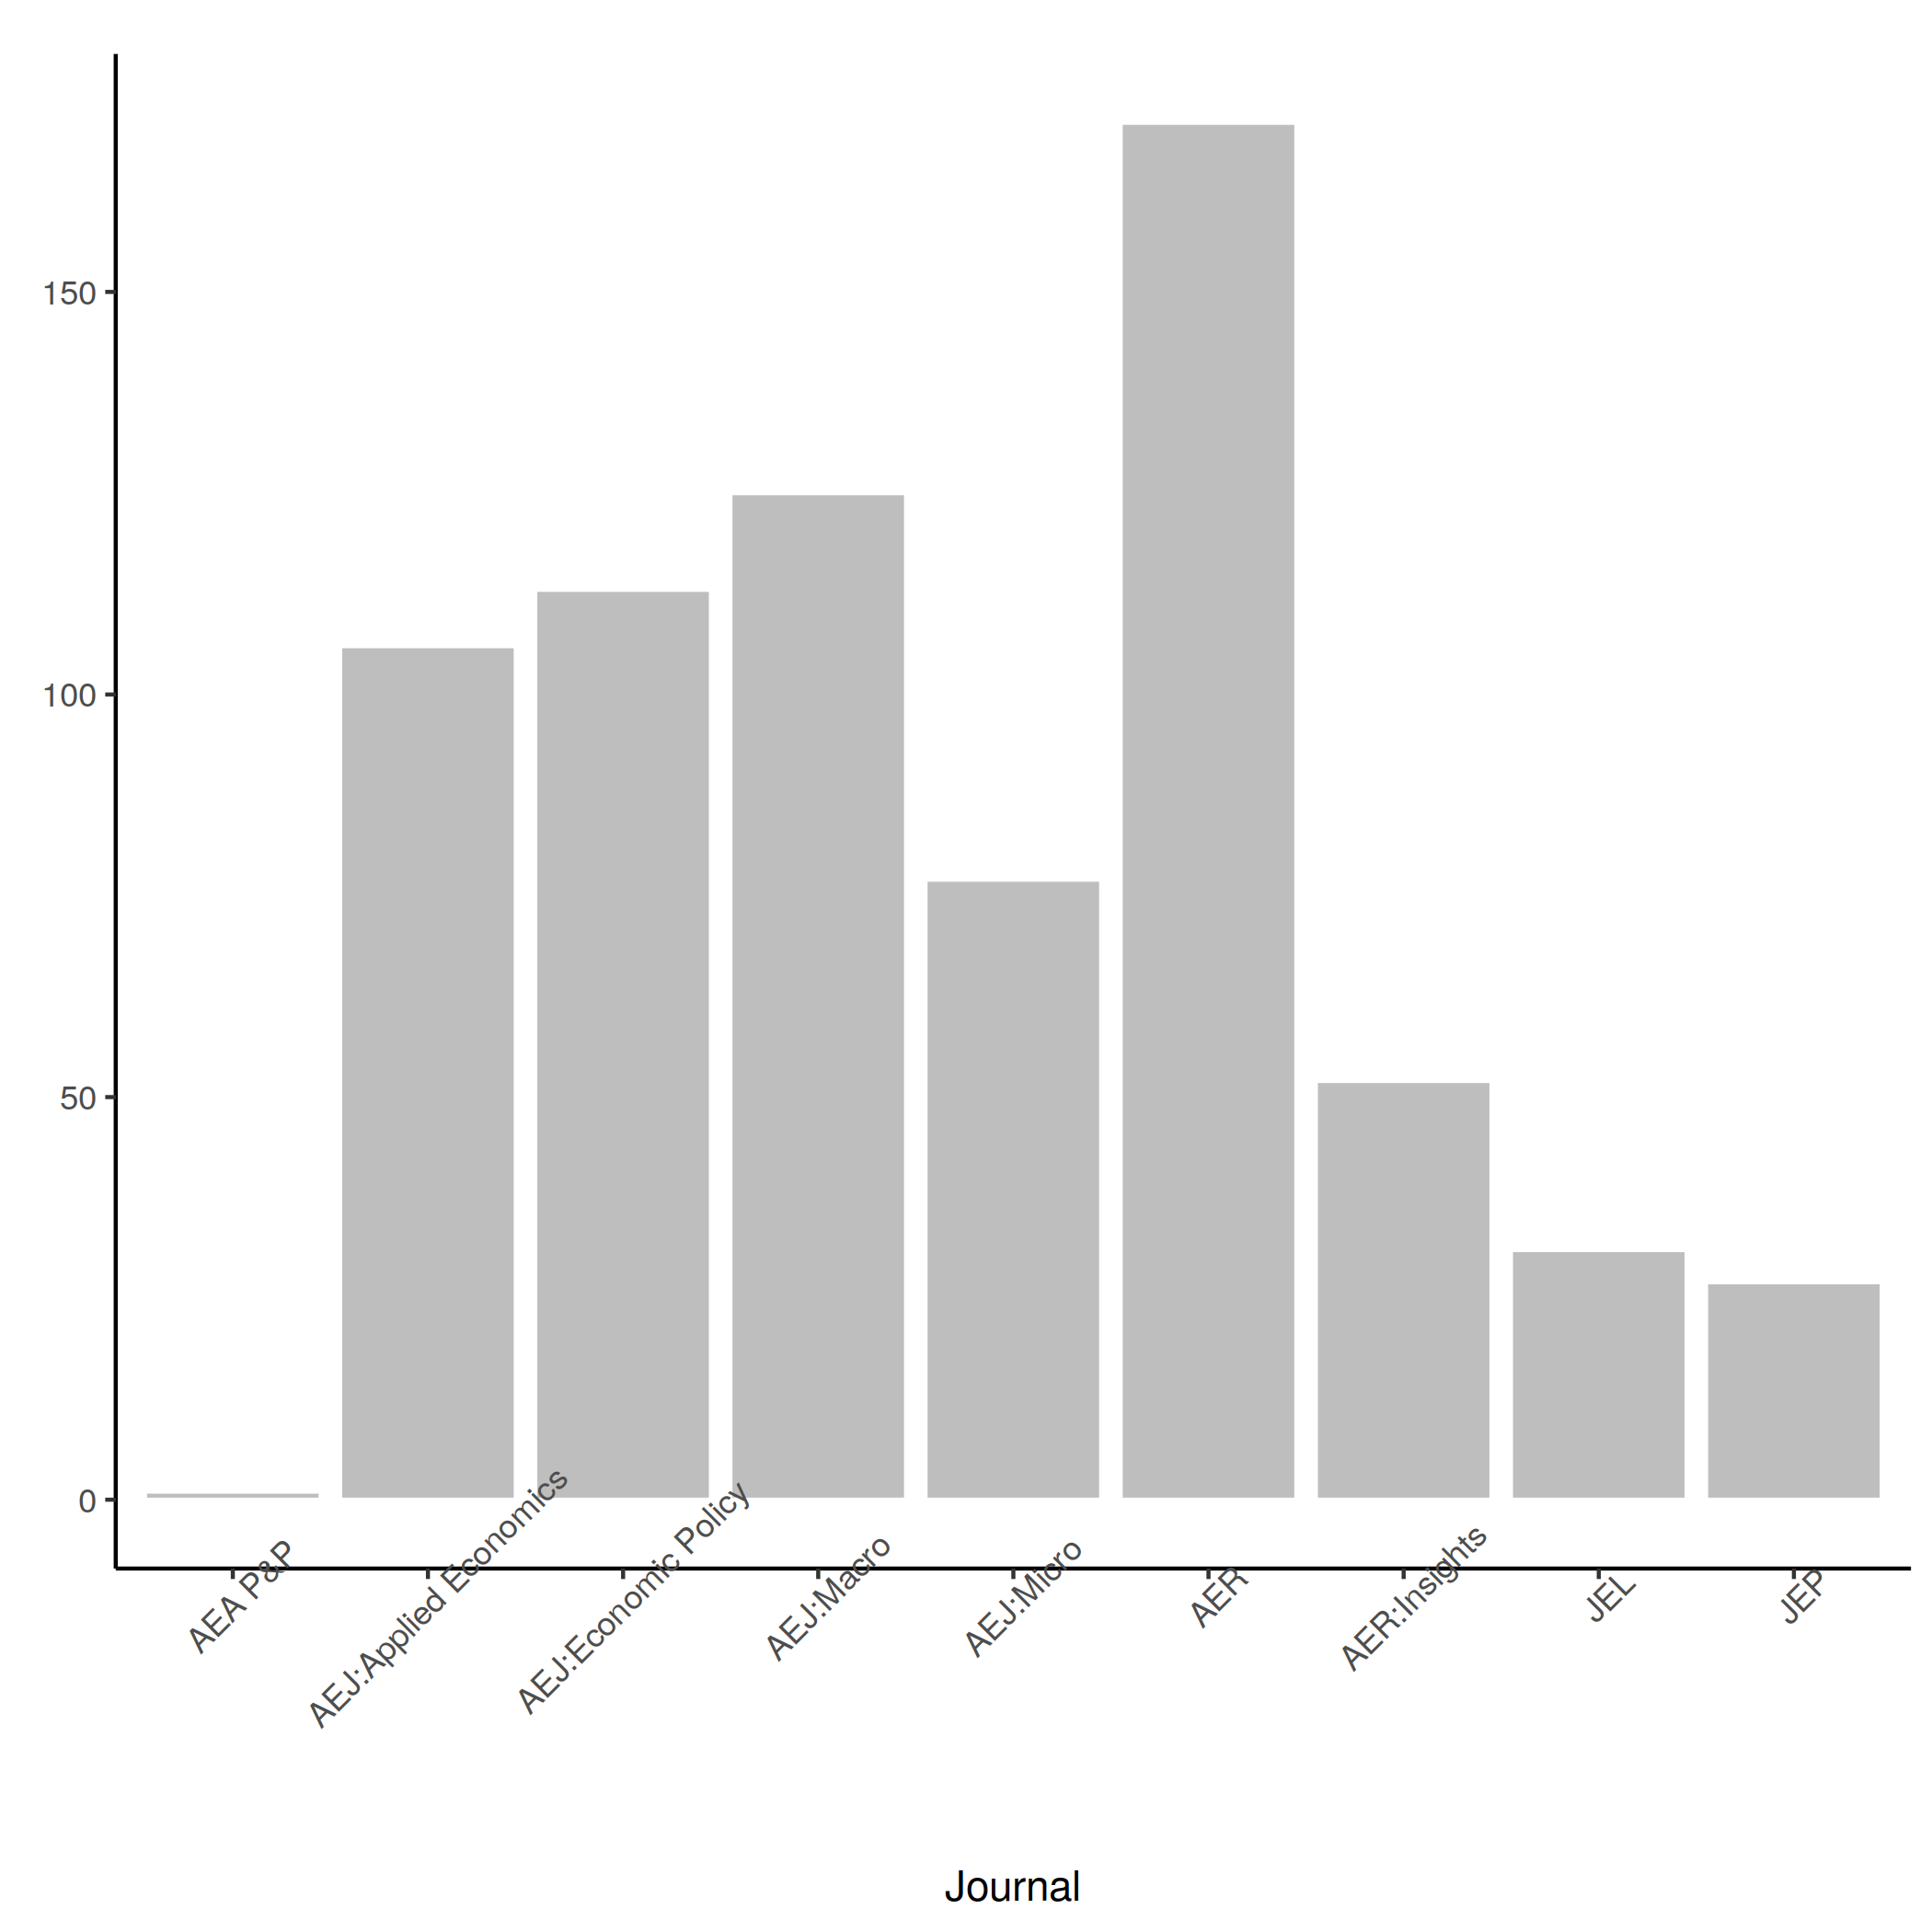
\includegraphics[height=0.4\textheight]{images/n_assessments_journal_plot.png}
    \caption{Number of assessments}
    \label{fig:pre:assessments_journal}
\end{figure}



\begin{figure}
    \centering
%    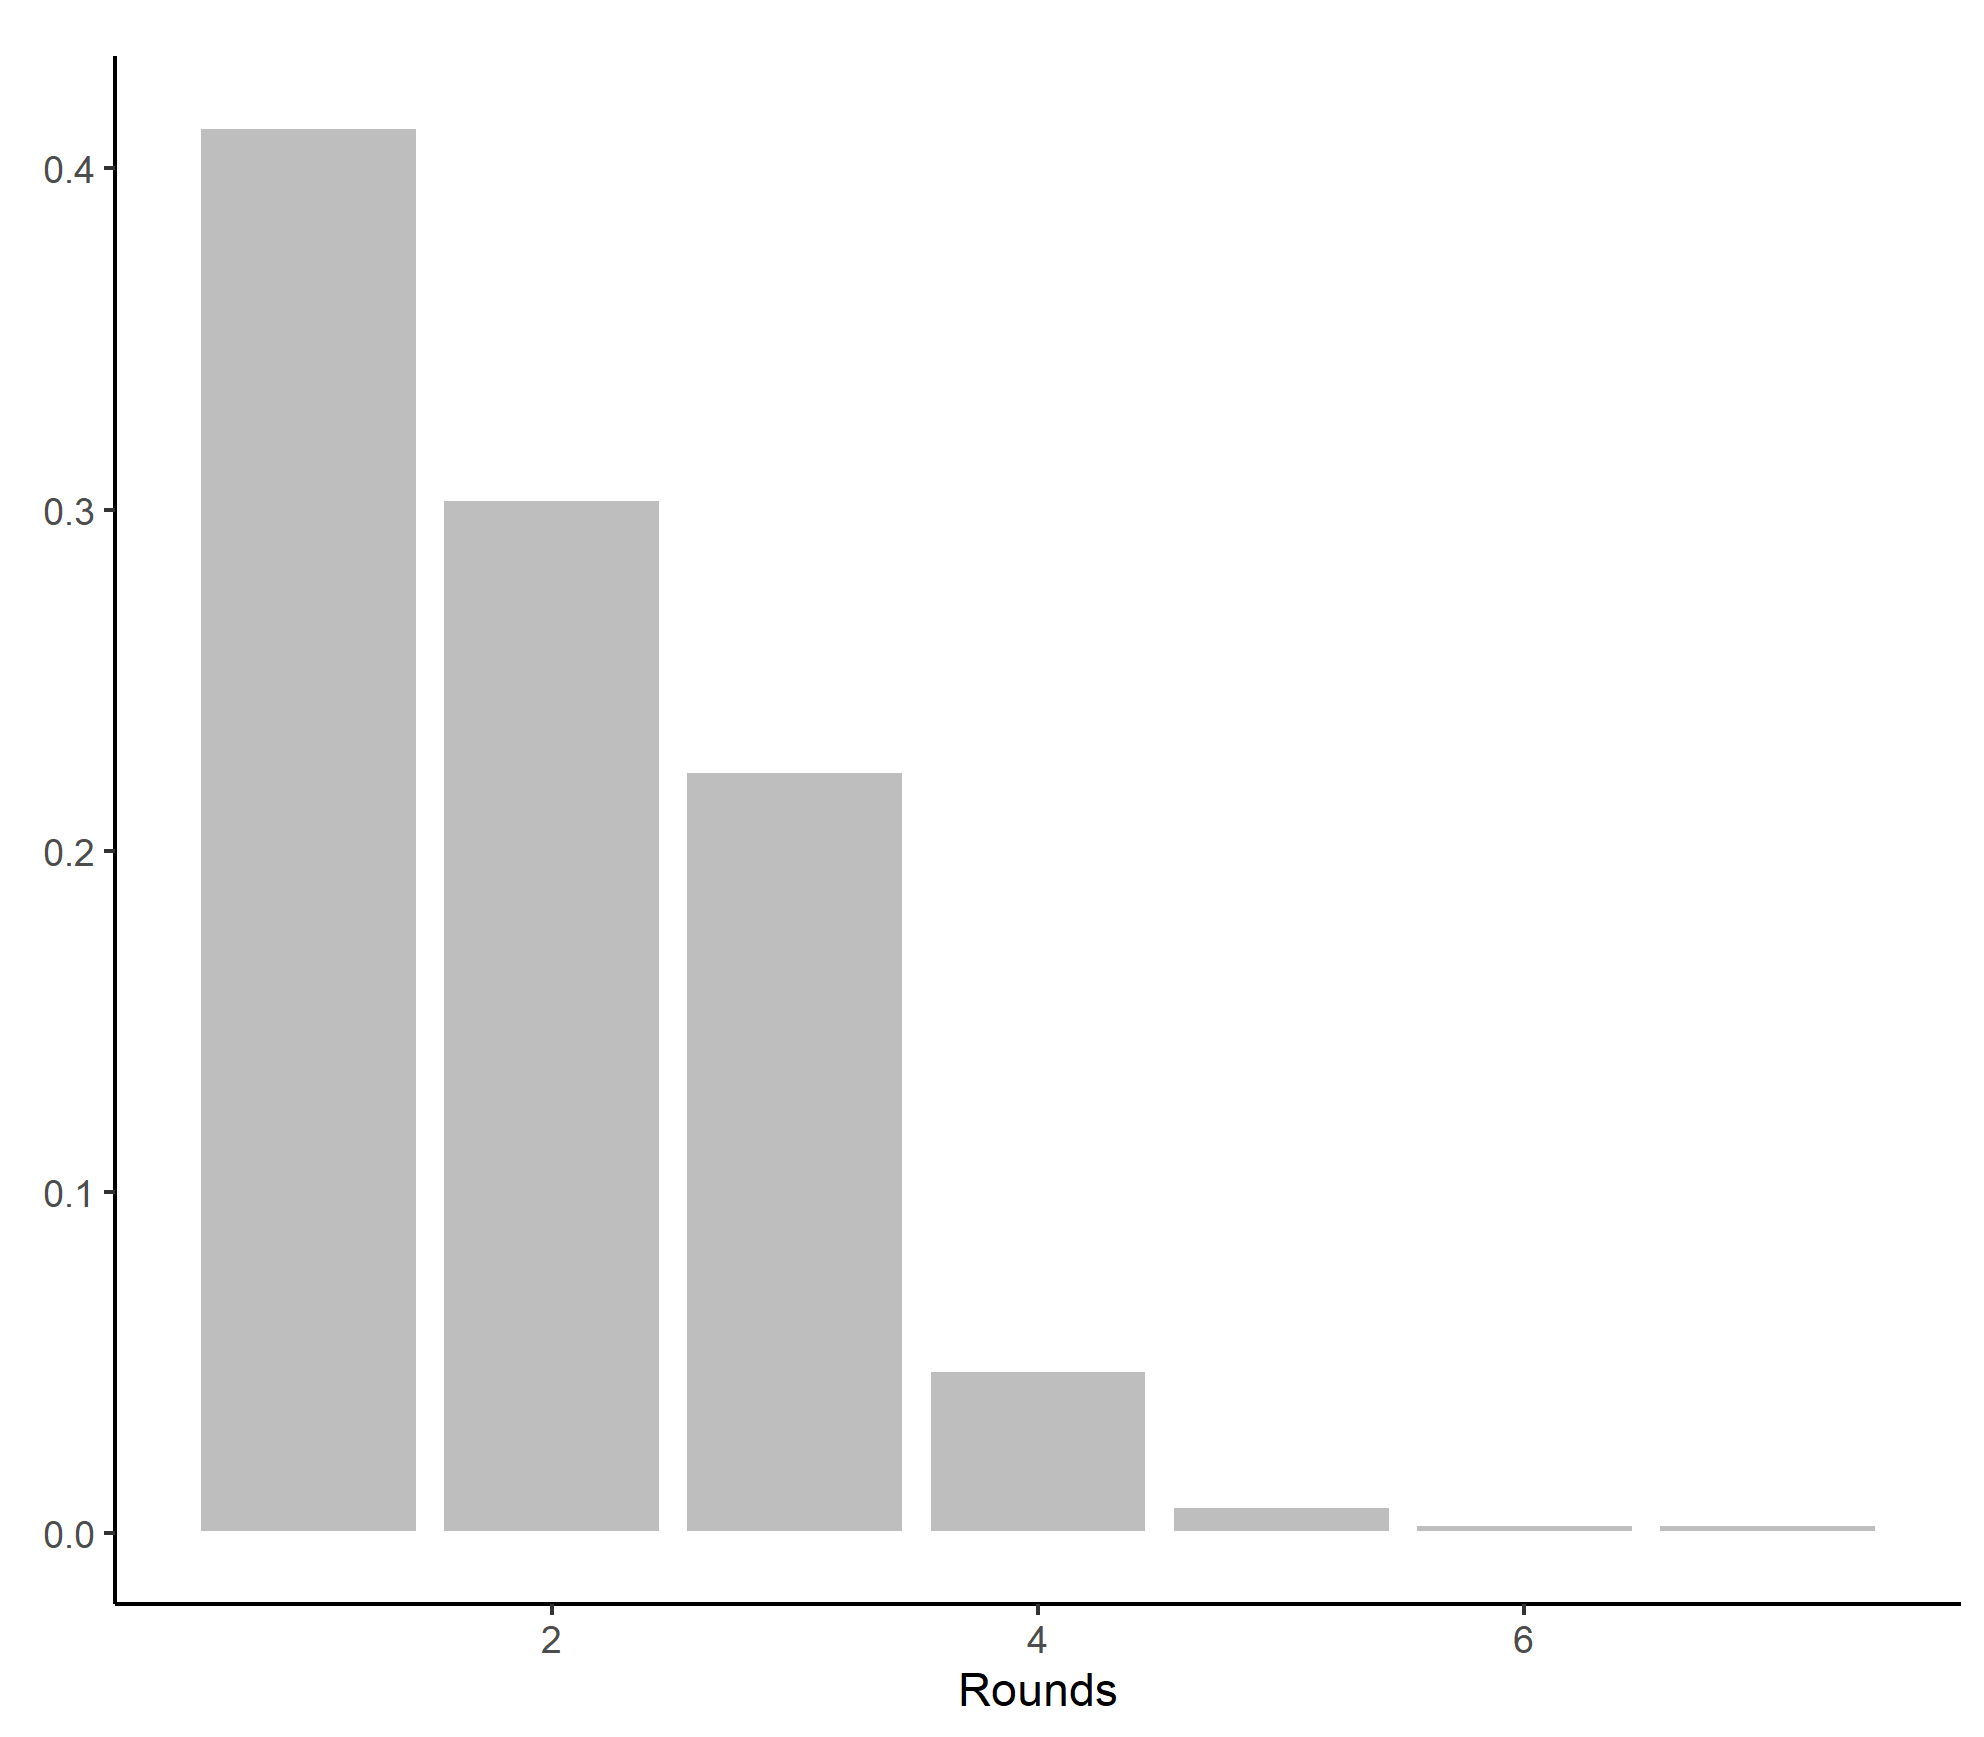
\includegraphics[height=0.4\textheight]{images/n_rounds_plot.png}
    \caption{Assessment rounds for completed manuscripts}
    \label{fig:pre:rounds}
\end{figure}

\begin{figure}
    \centering
%    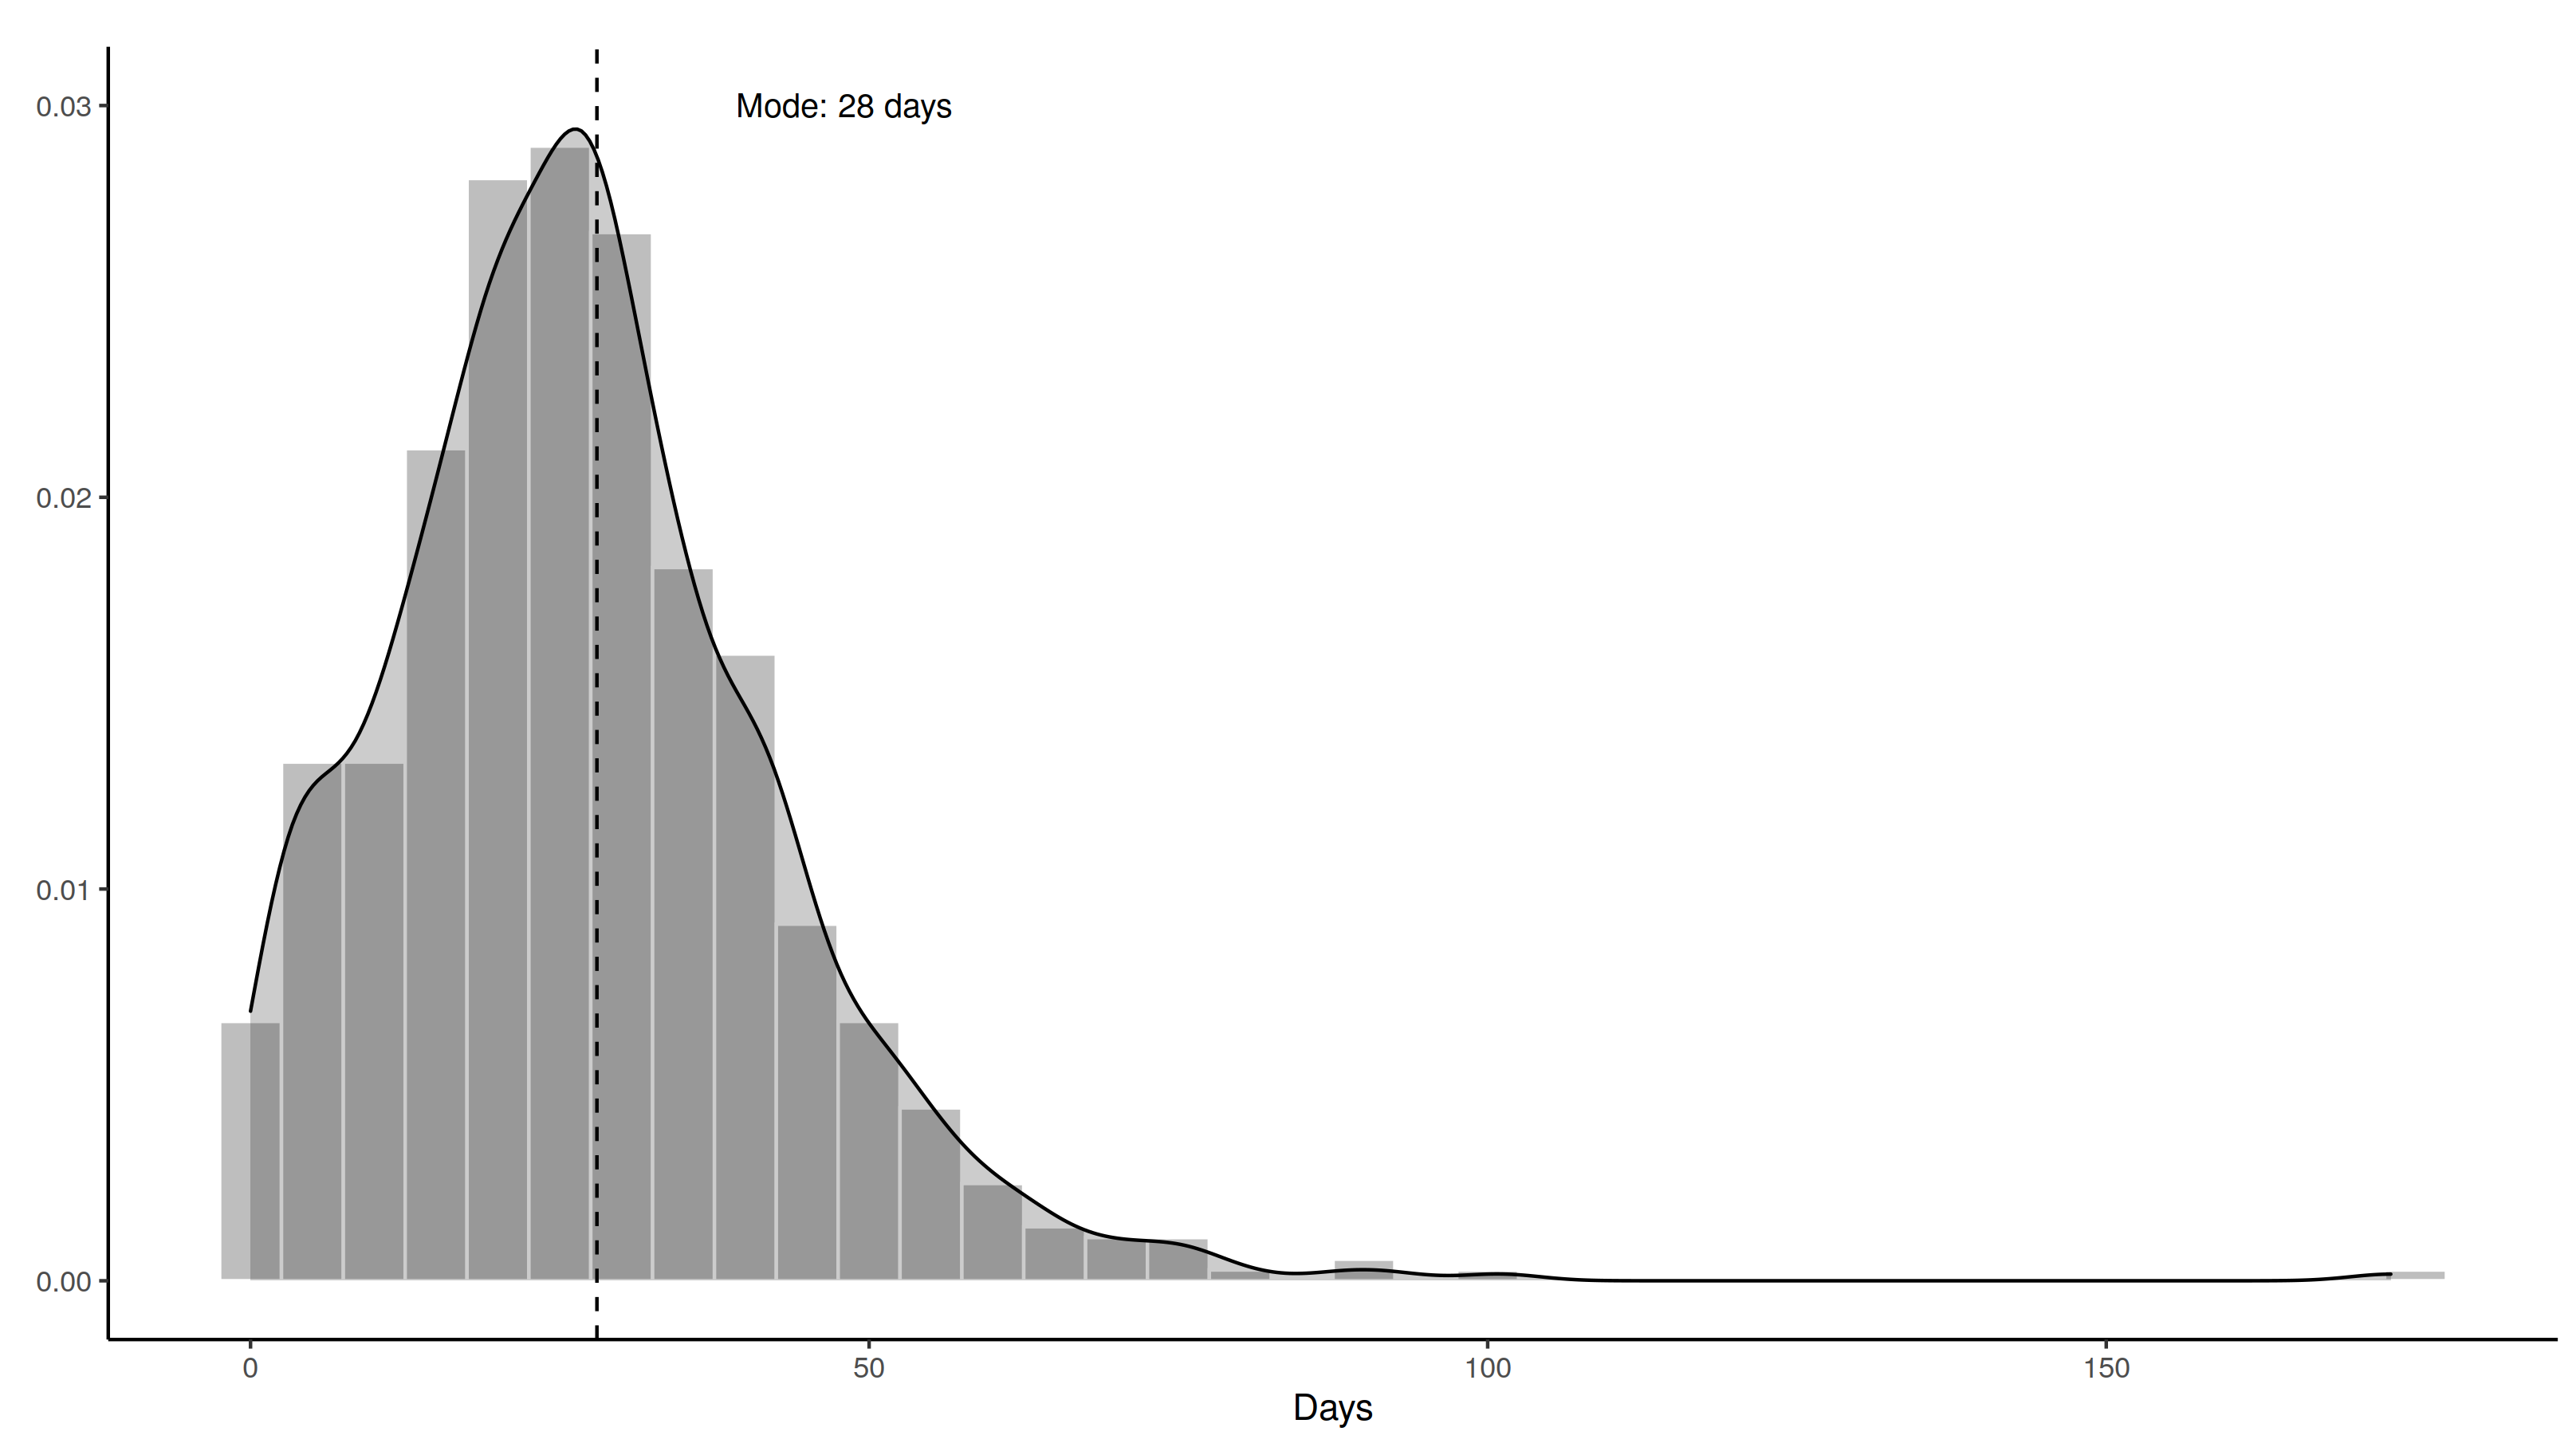
\includegraphics[height=0.4\textheight]{images/revision_round_length_hist.png}
    \caption{Length of an assessment round in days}
    \label{fig:pre:round_length}
\end{figure}

\begin{figure}
    \centering
%    \includegraphics[height=0.4\textheight]{images/total_length_hist.png}
    \caption{Length of revisions for completed manuscripts}
    \label{fig:pre:revision_length}
\end{figure}




\begin{figure}
    \centering
%    \includegraphics[height=0.4\textheight]{images/author_response_hist.png}
    \caption{Author response time}
    \label{fig:pre:author_response_time}
\end{figure}

\begin{quote}
    Issues with pre-publication verification
\end{quote}

\paragraph{Self-corrections}

We often find that authors find other errors than those the replication team identified. For instance, the manuscript figures might have come from an earlier version of the dataset, or from an earlier run of the code sequence with slightly different parameters. In other cases, while reviewing issues found by our replication team, authors correct econometric errors, which our process is not designed to find. 

\paragraph{Computational issues}

Numerical differences (Matlab versions, seeds) see \url{https://it.mathworks.com/matlabcentral/answers/
422349-fmincon-in-new-matlab-version-gives-different-results} as well. Cite the old papers. In some cases, the underlying feature leading to numerical differences is a subtle fragility of the optimization algorithm, or multiple distinct yet close optima that do not fundamentally affect the results.

Fortran challenges (manual compilation instructions, non-open source compile, no Makefiles, no parameter files).

GIS challenges (not considered use of "data", often not described at all, or mostly manual tasks when using ArcGIS - very little python with ArcGIS). 

Robustness checks that are manual

\paragraph{Delays} A recurring concern expressed by editors and staff members was the potential for   delays in publication, due to the verification process. The data presented here indicates that concerns of about a delay in the time-to-publication remain valid, though we have no evidence at this time that the overall time to publication has increased --- the first articles that completed the entire pre-publication verification process were published in late January 2020, after the analysis in this article was completed.

We are addressing these concerns in a variety of ways. First, the current set of manuscripts moving through the assessment process did not anticipate the process --- the manuscripts were written and refereed prior to the July announcement. They thus could not incorporate stronger guidance as easily as future submissions will be able to. Second, we are expanding guidance, as well as preparing template README and project structures that will assist future manuscript submissions to be more rapidly compliant with the \ac{DCAP}, ideally in a first pass. This may include stronger requirements about the information to be provided by authors, including detailed information about the length of time it takes to execute the computer code.
Third, there is anecdotal evidence that other factors affecting the time-to-publication have been reduced, due to the move to conditional acceptance. Thus, manuscript materials are being completed earlier than before. 

We note that none of the \jiramcs{} manuscripts we assessed had  fundamental flaws --- all problems identified so far have been fixable (and fixed). 





\section{Task 3: Working with Other Providers of Scientific Infrastructure to Improve Support for Documenting Provenance and Replicability}
\label{sec:coordination}

An important component of the AEA Data Editor's position is to interact with other providers of scientific infrastructure. This involves other publishers and journals, archives such as ICPSR, providers of restricted or proprietary data, the AEA RCT Registry, metadata harvesters, and third-party verification services. 
% for exec summary: Also briefing to staff members of the House and Senate Science committees.

\subsection{Highlighting Data Resources}

NEW: See Ganapati \url{https://www.aeaweb.org/articles?id=10.1257/mic.20190029} and Harari \url{https://www.aeaweb.org/articles?id=10.1257/aer.20171673} data extracts, deposits. Also 200GB of NASA data, IPUMS terms of use, citations, and conundrum of copying data when (easy) retrieval from the original provider is not possible.

\subsection{Economics Journals}

We have coordinated with other data editors conducting similar activities at other journals. In 2019, both the \ac{ReStud} and the \ac{EJ}  appointed data editors, tasked among other things with pre-publication verification. The \ac{CJE} is currently revising its \ac{DCAP}. The \ac{JASA} is expanding the scope of its pre-publication verification to all sections of the journal. In all cases, either the AEA Data Editor or an ad-hoc group of ``Social Science Data Editors'' initiate by the AEA Data Editor, was consulted. The ``Social Science Data Editors'' group includes  editors from journals that do not (yet) have a pre-publication verification service. A  \urlcite{socialsciencedataeditors.github.io}{website} provides examples, checklists, and links to training materials, to assist authors in  improving data and code archives prior to submission, regardless of the journal they may be submitting to.

\subsection{Search services, text mining access}
As noted earlier, the move of supplements into the openICPSR-supported repository enables broad dissemination of metadata on supplements. Among others, Google Dataset Search harvests and then displays such metadata. Staff from openICPSR and the AEA Data Editor have been discussing informally with the Google Dataset Search team on how to correctly display metadata as it moves through the various scrapers. 

Over the course of the past year, the AEA has been approached by two research projects that wished to use the full-text versions of AEA articles to enhance the linkage between articles and data. We worked with these teams to establish a policy by which they could legally access the full archive of articles, but also subsequently make their work available to others. AEA counsel is currently working on a full-fledged data and text mining policy.

\subsection{Third-party verification services}

\begin{quote}
    Write a lot here.
\end{quote}
We have started discussions with third-party verification services. In particular, we have trialled using their services, instead of our in-house team, to conduct assessments. This aligns with the discussions among editors about resources and scalability of assessments, and with the educational outreach, which some of these services also conduct. Part of the effort consists in aligning the criteria used by these services with those of the various journals.

\subsection{Commercial providers}

Highlight exemplary redistribution agreement at ESRI. Highlight in all cases the need to have access rights for pre-production verification, including to the same access mechanisms. 

\subsection{Non-commercial providers of restricted-access data}

Increased provision of data citations, clear license/ usage rights. Ongoing work. Briefings of US, Canadian, German, French, UK restricted access centers. Some providers have also reached out to inquire pro-actively how to improve their access mechanisms, distribution mechanisms, and documentation thereof.

\section{Task 4: Working with the Economics Community to Enhance and Broaden Education on Replicable Science}

\begin{quote}
    write about participation of other journals, as well as nascent efforts around Data-PASS and RDA.
\end{quote}

From the preliminary verification work has emerged a clear indication that education and training is critical for the adoption of reproducible methods. We are expanding the support materials, and are adapting them to each discipline's idiosyncratic methods. Training materials will be made available by various organizations, with input from the AEA Data Editor. The \urlcite{https://aeadataeditor.github.io/aea-de-guidance/}{AEA Data Editor's website} as well as the website of the \urlcite{https://social-science-data-editors.github.io/guidance/}{Social Science Data Editors} are being regularly updated with additional guidance, and will hopefully allow authors to be responsive to various journals' \ac{DCAP}.

\section{Data and Code Availability Statement}
\label{sec:dcas}

All data and code used to generate figures and tables in this article can be found at \citet{E117884V1}, with some data archived as \citet{E117873V1} and \citet{E117876V1}. Data on the AEA RCT Registry was extracted by JT and KW from internal systems, but can now be downloaded directly \citep{DVN/DFMLIU_2020}. The data provided here as part of \citet{E117884V1} may differ.

\FloatBarrier
% Remove or comment out the next two lines if you are not using bibtex.
%
% NOTE: Do not modify the AEADataEditor.bib manually!
%
\bibliographystyle{aea-mod}
\bibliography{paper,references}

% The appendix command is issued once, prior to all appendices, if any.
\appendix

%\input{appendix.tex}


\end{document}

